% chktex-file 13
%%%%%%%%%%%%%%%%%%%%%%%%%%%%%%%%%%%%%%%%%
% Stylish Article
% LaTeX Template
% Version 2.1 (1/10/15)
%
% This template has been downloaded from:
% http://www.LaTeXTemplates.com
%
% Original author:
% Mathias Legrand (legrand.mathias@gmail.com) 
% With extensive modifications by:
% Vel (vel@latextemplates.com)
%
% License:
% CC BY-NC-SA 3.0 (http://creativecommons.org/licenses/by-nc-sa/3.0/)
%
%%%%%%%%%%%%%%%%%%%%%%%%%%%%%%%%%%%%%%%%%

%----------------------------------------------------------------------------------------
%	PACKAGES AND OTHER DOCUMENT CONFIGURATIONS
%----------------------------------------------------------------------------------------

\documentclass[fleqn,10pt]{SelfArx} % Document font size and equations flushed left

\usepackage[ngerman]{babel} % Specify a different language here - english by default
\usepackage{csquotes}

\usepackage{lipsum} % Required to insert dummy text. To be removed otherwise

%----------------------------------------------------------------------------------------
%	COLUMNS
%----------------------------------------------------------------------------------------

\setlength{\columnsep}{0.55cm} % Distance between the two columns of text
\setlength{\fboxrule}{0.75pt} % Width of the border around the abstract

%----------------------------------------------------------------------------------------
%	COLORS
%----------------------------------------------------------------------------------------

\definecolor{color1}{RGB}{0,0,90} % Color of the article title and sections
\definecolor{color2}{RGB}{0,20,20} % Color of the boxes behind the abstract and headings

%----------------------------------------------------------------------------------------
%	HYPERLINKS
%----------------------------------------------------------------------------------------

\usepackage{hyperref} % Required for hyperlinks
\hypersetup{hidelinks,colorlinks,breaklinks=true,urlcolor=color2,citecolor=color1,linkcolor=color1,bookmarksopen=false,pdftitle={Title},pdfauthor={Author}}

%----------------------------------------------------------------------------------------
%	ARTICLE INFORMATION
%----------------------------------------------------------------------------------------

\JournalInfo{Handout, No. 1, \today} % Journal information
\Archive{Dieses Werk ist unter einer Creative Commons Lizenz vom Typ Namensnennung 2.0 Deutschland zugänglich. Um eine Kopie dieser Lizenz einzusehen, konsultieren Sie http://creativecommons.org/licenses/by/2.0/de/ oder wenden Sie sich brieflich an Creative Commons, Postfach 1866, Mountain View, California, 94042, USA.} % Additional notes (e.g. copyright, DOI, review/research article)

\PaperTitle{12 Factor App} % Article title

\Authors{Sidney Kuyateh\textsuperscript{1}, Steffen Walter\textsuperscript{2}} % Authors
\affiliation{\textsuperscript{1}\textit{Studiengang Informationstechnik, Fakultät Technik, Duale Schule Baden-Württemberg, Stuttgart}} % Author affiliation
\affiliation{\textsuperscript{2}\textit{Studiengang Informationstechnik, Fakultät Technik, Duale Schule Baden-Württemberg, Stuttgart}} % Author affiliation
\affiliation{*\textbf{Corresponding author}: inf17001@lehre.dhbw-stuttgart.de} % Corresponding author

\Keywords{} % Keywords - if you don't want any simply remove all the text between the curly brackets
\newcommand{\keywordname}{Keywords} % Defines the keywords heading name

%----------------------------------------------------------------------------------------
%	ABSTRACT
%----------------------------------------------------------------------------------------

\Abstract{Das vorliegende Handout soll einen kurzen Überblick über die Kriterien geben, welche bei der Erstellung einer Web-Applikation unter den Vorgaben der \enquote{12 Factor App} beachtet werden müssen.\newline Mit der \enquote{12 Factor App} hat Adam Wiggins von der Firma Heroku im Jahr 2011 eine Methode vorgestellt, mit der sich Software-As-A-Service (SaaS) Apps entwerfen und umsetzten lassen, die folgenden Kriterien entsprechen:
\begin{itemize}
	\item Deklarative Formate zur Kosten- und Zeitoptimierung
	\item Klare Schnittstellen zum Betriebssystem für maximale Portabilität
	\item Deploymentmöglichkeiten für modernen Cloudplattformen
	\item Minimierung des Wegs von der Entwicklung zum produktiven Einsatz, für maximale Agilität
	\item Die Möglichkeit zur einfachen Skalierung, ohne weitreichende Änderungen
\end{itemize}}

%----------------------------------------------------------------------------------------

\begin{document}

\flushbottom % Makes all text pages the same height

\maketitle % Print the title and abstract box

%\tableofcontents % Print the contents section

\thispagestyle{empty} % Removes page numbering from the first page

%----------------------------------------------------------------------------------------
%	ARTICLE CONTENTS
%----------------------------------------------------------------------------------------

\section*{Einleitung} % The \section*{} command stops section numbering

\addcontentsline{toc}{section}{Introduction} % Adds this section to the table of contents
Die Entwickler der 12 Factor App stammen von der Firma Heroku, wo sie der Entwicklung zahlreicher Webapplikationen im Bereich SaaS beigewohnt haben, um dann die Synthese ihrer Erfahrungen in einem Dokument zusammen zu fassen und zu Veröffentlichen.\newline
Das Ziel dabei ist es, dass SaaS Apps künftig einfacher skalierbar sind, besser durch ein Team gepflegt und auf Dauer mit kalkulierbaren Kosten weiterentwickelt werden können. Das Konzept richtet sich gleichermaßen an Entwickler wie auch an Administratoren, die mit dem Deployment betraut sind.

%------------------------------------------------

\section{Die Zwölf Faktoren}
Eine \enquote{12 Factor App} benötigt wie der Name schon vermuten lässt zwölf Faktoren um den formulierten Ansprüchen zu genügen. Im Folgenden werden diese Faktoren kurz vorgestellt. 
\subsection{I. Codebase}
Um dem Anspruch einer \enquote{12 Factor App} zu genügen muss der Code immer durch ein Versionsmanagement wie Git oder SVN verwaltet werden. Dabei wird die jede Änderung in einer Versionsdatenbank gespeichert.\newline
Weder mehrere Repositories noch duplizierter Code in verschiedenen Repositories ist zulässig. Verschiedene Codebases sind als mehrere Apps zu behandeln und duplizierter Code muss in Bibliotheken ausgelagert werden.
\subsection{II. Abhängigkeiten}
Die meisten Anwendungen sind abhängig von externen Bibliotheken welche sowohl global, wie auch im Verzeichnis der App zu Verfügung stehen können. Um den Kriterien der \enquote{12 Factor App} zu entsprechen müssen Bibliotheken unabhängig von der Plattform, auf welcher die Anwendung ausgeführt wird, zur Verfügung stehen. Es ist folglich nicht zulässig systemweite Bibliotheken zu verwenden. Weiterhin ist es erforderlich Maßnahmen zu ergreifen, die Sicherstellen, dass die Bibliotheken verschiedener Anwendungen von einander isoliert werden.\newline
Es ist außerdem nicht davon auszugehen, dass bestimmte Systemwerkzeuge zur Verfügung stehen.
\subsection{III. Konfiguration}
Konfigurationen sind zwingend außerhalb der Codebase zu definieren. Es muss sichergestellt sein, dass es nicht zu einer Vermischung von Quellcode und Konfiguration kommt. Um dies zu gewährleisten sind Umgebungsvariablen zu verwenden. Bei der Verwendung von Umgebungsvariablen ist darauf zu achten, dass diese immer universell einsetzbar sein müssen und nicht an spezielle Umgebungen gebunden sein dürfen.
\subsection{IV. Unterstützende Dienste}
Unter einem unterstützenden Dienst wird jeder nachgelagerte Dienst verstanden der über Netzwerk an die Applikation \enquote{angedockt} werden kann. Es wird nicht zwischen Cloud- und On-Premises-Diensten unterschieden. Auch wenn mehrere Dienste die gleiche Funktion bieten werden sie als eigenständiger Dienst begriffen. Dem Modularen System entsprechend soll es möglich sein unterstützende Dienste beliebig an- und abzuhängen, ohne dass Änderungen am Quellcode vorgenommen werden müssen.
\subsection{V. Build, Release, Run}
Um vom Quellcode einer Anwendung zu einem laufenden System zu kommen sind drei Schritte nötig:
\begin{enumerate}
	\item Die Build-Pase, in welcher der Quellcode in ausführbaren Code transformiert wird. Gegebenefalls muss er zu diesem Zweck kompiliert werden.
	\item In der Release-Phase wird die Anwendung mit der nötigen Konfiguration ausgestattet um in der gewünschten Umgebung lauffähig zu sein.
	\item Die Run-Phase zeichnet sich dadurch aus, dass alle nötigen Prozesse auf dem Zielsystem gestartet werden, um den vollen Funktionsumfang der Anwendung zur Verfügung zu stellen.
\end{enumerate}
Änderungen können nicht zur Laufzeit vorgenommen werden, stattdessen werden sie durch neue Releases dem System zugeführt. Es bietet sich an hierfür ein eine Release-Verwaltung einzusetzen um bei Fehlern in neuen Releases ohne großen aufwand zu einem vorherigen Release zurück zu kehren.
\subsection{VI. Prozesse}

%Sidney
\subsection{VII. Bindung an Ports}
Die Zwölf-Faktor-App läuft eigenständig und unabhängig von einem gegebenfalls vorhandenem Webserver. Die Verarbeitung von HTTP-Requests und -Responses verläuft vollständig innerhalb des Appcodes. Dazu bindet sich die App an einen Port und wartet dort auf Requests. Auch andere Protokolle können über diese Methode angeboten werden.
\subsection{VIII. Nebenläufigkeit}
Die Zwölf-Faktor-App wird anhand der Anzahl laufender Prozesse skaliert. Anstatt von pid-Dateien und Daemons wird der Prozessmanager des Betriebssystems verwendet, um abgestürtzte Prozesse und vom Nutzer initiierte Neustarts zu verwalten.
\begin{figure}[htpb]
	\centering
	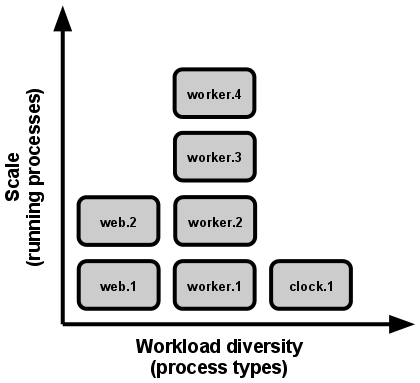
\includegraphics[width=0.3\textwidth]{../process-types.png}
	\caption{Skalierung mit Prozessen~\cite{factor-concurrency}}
\end{figure}
\subsection{IX. Entsorgbarkeit}
Die Prozesse der Zwölf-Faktor-App sind jederzeit entsorgbar, d.h.\@ die Prozesse können jederzeit gestartet und beendet werden. Deshalb ist sehr wichtig, dass möglichst kleine Startzeiten und ein möglichst unproblematisches Beenden möglich sind. Außerdem muss die App robust gegenüber plötzlichen Tod sein, sodass keine Datenverluste auftreten. Auf die Spitze getrieben wäre ein mögliches Crash-only design.
\subsection{X. Dev-Prod-Gleichheit}
Die Zwölf-Factor-App hat möglichst gleiche Entwicklungs- und Produktionsumgebungen. Die Zwölf-Factor-App ist für Continuous Deployment ausgelegt, was bedeutet, dass die Verteilung einer neuen Version innerhalb von Stunden geschieht. Gleiche Hintergrunddienste in beiden Umgebungen sind dabei wichtig, um eventuelle Inkompatibilitäten schon bei der Entwicklung erkennen zu können.
\subsection{XI. Logs}
Die Zwölf-Factor -App sieht Logs als Eventströme. Die Zwölf-Faktor-App kümmert sich nicht um das Ziel der Ausgabedate, sondern es wird immer nach \texttt{stdout} geschrieben. Die Ausführungsumgebung sammelt die Ausgaben aller Prozesse und kümmert sich um das Verarbeiten. Dadurch besteht die Möglichkeit, spezielle Loganalyse und -indizierungssysteme zu verwenden, welche das Aufspüren von Problemen effizienter zu gestalten.
\subsection{XII. Administrationsprozesse}
Die Zwölf-Factor-App hat Administrationen als einmalige Vorgänge. Wichtig ist wieder, dass auch administrative Aufgaben in derselben Umgebung wie die App laufen. Sie laufen in derselben Isolationsebene (Bundler bei Ruby, virtualenv bei Python etc.), um Inkompatibilitäten zu vermeiden. Administrativer Code wird auch gemeinsam mit dem Anwendungscode ausgeliefert, um Synchronisationsprobleme mit verschiedenen Versionen vorzubeugen.
\section{Fazit}
Die 12 Factor App hat auch noch Schwächen. Es wird als eine gute Basis für die Entwicklung von Web Apps gesehen. Allerdings gibt es auch Kritik an dem Modell. Kritik kommt unter anderem von Kevin Hoffman, wieder diese in dem Buch \enquote{Beyond the 12 Factor App}~\cite{beyond} beschrieben hat. Er erweitert die 12 Faktoren auf 15 und überarbeitet die vorhandenen Faktoren. Insbesondere äußert er Kritik am fehlenden Faktor Sicherheit, welches zentraler Bestandteil einer Web App sein muss. Aös weiteren Ansatz gibt er das Prinzip \enquote{API first} an, welches eine bessere Integration in Systeme und Apps erlaubt. Als weiterer Punkt nimmt er die Telemetrie, welche es erlaubt, die App weiter auf das Nutzerverhalten zu optimieren.

%\begin{figure}[ht]\centering % Using \begin{figure*} makes the figure take up the entire width of the page
%
\includegraphics[width=\linewidth]{view}
%\caption{Wide Picture}
%\label{fig:view}
%\end{figure*}


%------------------------------------------------

%----------------------------------------------------------------------------------------
%	REFERENCE LIST
%----------------------------------------------------------------------------------------
\phantomsection%
\bibliographystyle{unsrt}
\bibliography{../literatur}

%----------------------------------------------------------------------------------------

\end{document}